\subsection{HTTP (Weiland)}

Das "'Hypertext Transfer Protocol"' ist ein Protokoll des Application Layers des OSI-Layer-Modells.
\\
HTTP ist ein zustandsloses Protokoll. Anfragen werden stets getrennt behandelt, auch wenn sie vom selben Client stammen. Dies kann durch eine Session geändert werden.
\subsubsection{Verbindungsvorgang}
Zu Beginn wird die Zieladresse in eine IP-Adresse umgewandelt.
Anschließend wird eine TCP-Verbindung  mit dem Server aufgebaut. 
Dann wird eine Anfrage an den Port 80 des Server gesendet.
\\
\begin{lstlisting}[style=custom, caption={HTTP-Request},label={lst:content_http_request}]
GET / HTTP/1.1\r\n
Host: htlinn.ac.at\r\n
User-Agent: Mozilla/5.0 (Windows NT 6.1; WOW64; rv:28.0) Gecko/20100101 Firefox/28.0\r\n
Accept: text/html,application/xhtml+xml,application/xml;q=0.9,*/*;q=0.8\r\n
Accept-Language: de,en-US;q=0.7,en;q=0.3\r\n
Accept-Encoding: gzip, deflate\r\n
Connection: keep-alive\r\n
\r\n
\end{lstlisting}

\begin{description}
\item[GET] Gibt an welche Datei aufgerufen werden soll. Da nach dem \enquote{/} kein Dateiname steht, wird die Seite aufgerufen, die beim Webserver als Standardseite eingetragen ist.
\item[Host] Als Host wird die Adresse des gewünschten Servers eingetragen. Sie wird in eine IP-Adresse umgewandelt und dem TCP übergeben. Muss seit Einführung von HTTP/1.1 vorhanden sein, da ansonsten der Statuscode \enquote{400 Bad Request} zurückgesendet wird.
\item[User-Agent] Der User-Agent ist jene Anwendung, die diesen Request ausgelöst hat. In diesem Fall der Browser Mozilla Firefox Version 28.0.
\item[Accept] Dies dient zur Übermittlung der erlaubten Dateiformate. Falls der Server keinen der angegebenen Dateitypen unterstützt, muss er mit dem Fehlercode \enquote{406 Not acceptable} antworten. Wird dieses Feld nicht in den Header eingetragen, so wird jeder Typ unterstützt.
\item[Accept-Language] Gibt an welche Sprachen die aufgerufene Seite haben soll. Wenn auf dem Server verschiedene Sprachen vorhanden sind, wird die gewünschte ausgegeben. In diesem Fall sollte dies Deutsch oder Englisch(USA) sein. 
\item[Accept-Encoding] Gibt die akzeptierten Kompressionsarten z.B. gzip an. Dies dient dazu, eine schnellere Übermittlung der Daten zu ermöglichen.
\end{description} 
Sobald zwei aufeinander folgende Zeilenenden erreicht wurden, beginnt der Server die Anfrage zu bearbeiten.

\begin{lstlisting}[style=custom, caption={HTTP-Response},label={lst:content_http_response}]
HTTP/1.1 200 OK\r\n
Date: Mon, 14 Apr 2014 13:38:48 GMT\r\n
Server: Apache/1.3.33 (Unix) FrontPage/5.0.2.2623 PHP/4.3.10 mod_perl/1.29\r\n
X-Powered-By: PHP/4.3.10\r\n
Connection: close\r\n
Transfer-Encoding: chunked\r\n
\r\n
\end{lstlisting}
\begin{description}
\item[Statuscode] siehe Statuscodes
\item[Date] Zeit, zu der der Response versendet wurde.
\item[Server] Äquivalent zu User-Agent für den Client. Gibt den verwendeten Server an. 
\item[X-Powered-By (nicht standardisiert)] Gibt die verwendete Technologie, in diesem Fall PHP Version 4.3.10, an. 
\item[Connection] Die bevorzugte Verbindungsart.
\item[Transfer-Encoding] Kompressionsverfahren mit welchem die zu übertragenden Daten komprimiert bzw. aufgeteilt wurden.
\end{description}
\autoref{lst:content_http_request} und \autoref{lst:content_http_response} wurden mittels Wireshark aufgenommen.
\subsubsection{Statuscodes}
Es gibt für HTTP sechs verschiedene Arten von Satuscodes
\paragraph{1xx}
Diese Statuscodes werden während der Bearbeitung der Anfrage verwendet und dienen der Information.
\paragraph{2xx}
Diese Statuscodes werden benützt, wenn die Anfrage erfolgreich bewältigt wurde.  
\paragraph{3xx}
Diese Codes dienen dazu, eine Umleitung ersichtlich zu machen. Bei solch einem Code wird eine Aktion des Clients gefordert, was meist automatisch geschieht. So wird zum Beispiel bei dem Statuscode \enquote{301 Moved Permanently} die neue Adresse im Header im Feld Location zurückgegeben.
\paragraph{4xx}
Hiermit werden Fehler gekennzeichnet. Zum Beispiel 404: "Not Found".
\paragraph{5xx}
Diese Codes sollen Server-Fehler kennzeichnen.

\subsubsection{Versionen}
Aktuell sind zwei verschiedene Versionen von HTTP im Einsatz, HTTP/1.0 und HTTP/1.1.
\\
Diese unterscheiden sich insofern, dass bei HTTP/1.0 für jede Anfrage eine neue Verbindung zum Server aufgebaut wird. Dies wirkt sich nachteilig auf die Geschwindigkeit aus, da, z.B. auf einer Website mit vielen Bildern, für jedes Bild eine neue Verbindung hergestellt werden muss und diese Verbindungen durch die Eigenschaften von TCP-Verbindungen (z.B. Slow-start ) entsprechend langsam sind.

\paragraph{HTTP/2.0}  HTTP/2.0 befindet sich in der Entwicklung und basiert auf SPDY. Es wird von der \enquote{Hypertext Transfer Protocol Bis working group}, einer Arbeitsgruppe der \enquote{Internet Engineering Task Force} (IETF), entwickelt.

\subsection{HTTPS (Weiland)}
HTTPS (= Hypertext Transfer Protocol Secure) dient zur Verschlüsselung der Verbindung von Client zu Server. Dies geschieht mittels SSL/TLS.
\subsubsection{Verbindungsaufbau}
Zuerst wird eine Authentifizierung und eine Identifizierung der Kommunikationspartner durchgeführt. Dann wird ein symmetrischer Schlüssel \enquote{ausgemacht}. Für diesen Vorgang kann entweder eine asymmetrische Verschlüsselung oder der \enquote{Diffie-Hellman-Merkle-Schlüsselabtauch} verwendet werden. Dies soll gewährleisten, dass nur die beiden Kommunikationspartner die Verschlüsselung kennen.
\subsubsection{Zertifikate}
Für SSL wird ein digitales Zertifikat benötigt, welches von einer Zertifizierungsstelle ausgestellt wird.
\paragraph{Erhalten eines Zertifikats}
Um ein Zertifikat zu erhalten, muss bei einer Zertifizierungsstelle darum angesucht werden. Zunächst wird eine E-Mail an den Betreiber der Domain gesendet.
\begin{figure}[H]
\centering
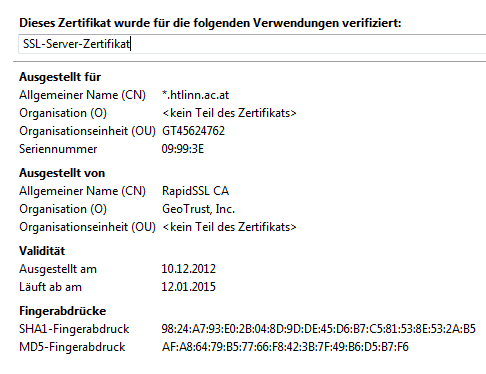
\includegraphics[keepaspectratio=true, width=12cm]{images/screenshots/certificate.png}
\caption{Allgemeine Zertifikatinforamtionen}
\label{fig:certificate}
\end{figure}
Die meisten Browser haben standardmäßig eine Liste von Zertifizierungsstellen eingetragen, welchen sie vertrauen. Diese Liste kann vom User jederzeit erweitert werden, jedoch sollte der User sich bezüglich der Seriosität der Zertifizierungsstelle wirklich sicher sein. 

\subsubsection{Sicherheitsprobleme}
Eine Schwachstelle der oben genannten Arten des Schlüsseltausches ist jedoch ein Man-in-the-Middle. Dieser müsste vor Aufbau der Verbindung von Host1 und Host2 zwischen ihnen liegen. In Folge würde er jeweils mit Host1 und Host2 eine Verschlüsselung ausmachen. Wenn er nun die gesendeten Daten von Host1 an Host2 weiterleitet und umgekehrt, können die beiden Hosts dies nicht bemerken.\\
Jedoch benötigt der Man-in-the-Middle ebenso ein Zertifikat, in dem steht, dass er der Zielserver sei. Um dies zu bewerkstelligen, muss der Angreifer Zugang zu einer Zertifizierungsstelle besitzen und sich ein Zertifikat ausstellen lassen.